%pbssm
\documentclass[../../main/main.tex]{subfiles}




\begin{document}
\title{Patrol Base Operations as Secure State Machines}


%%%%%%%%%%%%%%%%%%%%% Chapter PB SSM %%%%%%%%%%%%%%%
\chapter{Patrol Base Operations as Secure State Machines} \label{chp:pbssm}
The hierarchy of secure state machines (\glsentryshortpl{ssm}) consists of many \glsentryshortpl{ssm}.  Ten of these \glsentryshort{ssm} are verified in \glsentryshort{hol}.  Many of these \glsentryshortpl{ssm} are similar.  Thus, a sampling of representative \glsentryshortpl{ssm} is described in this section.  All \glsentryshortpl{ssm} can be found in the appendices starting with appendix \ref{app:ssms}.  They are also contained in the MasterThesis/HOL/ folders.

      %%%%%%%%%%%%%%%%%%% Section ssmPB %%%%%%%%%%%%%
\section{ssmPB: A Typical Example from the Hierarchy}\label{sec:ssmpb}
ssmPB is the top level \glsentryshort{ssm}.  It is an example of a typical one-principal \glsentryshort{ssm}.  A diagram of ssmPB is shown in figure \ref{ssmPBDiagram2}.


\begin{figure}[h!]
\centering
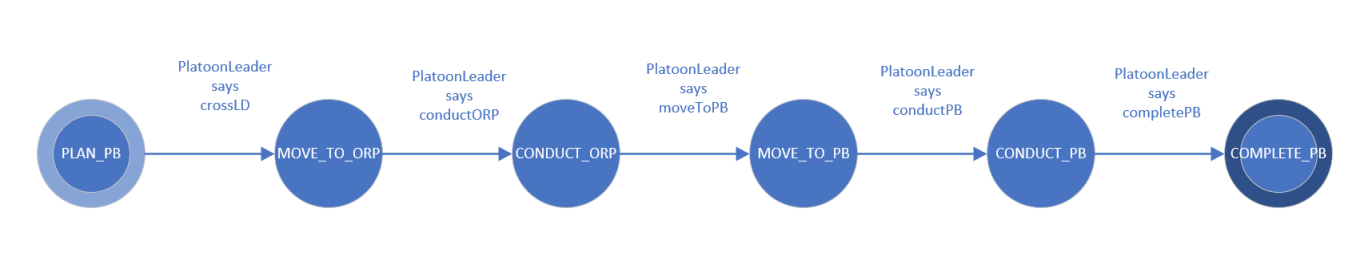
\includegraphics[width=\textwidth]{../figures/ssmPBDiagram}
\caption{\label{ssmPBDiagram2} Top level diagram.}
\end{figure}

ssmPB runs sequentially from the initial state PLAN_PB to the final state COMPLETE_PB.  State transitions require notification from the Omni principal that the state is complete and a request from the Platoon Leader to change states.  Thus, a transition request has the form 
\[\text{\textit{Omni says stateComplete}};\]
\[\text{\textit{PlatoonLeader says moveToNextState}}\]  

The security context reflects this two input requirement.  It authorizes the Platoon Leader on \textit{moveToTheNextState} if the current state is complete. A clause in the security context has the form
\[\text{\textit{stateComplete impf}}\]
\[\text{\textit{PlatoonLeader controls moveToNextState}}\]  

This clause is state dependent because \textit{stateComplete} is specific for the current state.  Thus, there are five statements in the state-dependent security context.

There is also a state-independent security context.  This has one clause authorizing the Omni principal on all omniCommands.   It has the form
\[\text{\textit{Omni controls stateComplete}}\]

Both the Omni and PlatoonLeader principals are authenticated on all slComands.  This includes omniCommands and plCommands.  However, authorization does distinguish between omniCommand and plCommand.  The authentication function has two statements of the form
\[\text{\textit{Omni says slCommand}}\]
\[\text{\textit{PlatoonLeader says slCommand}}\]  

The \glsentryshort{hol} implementation of the datatypes, functions, and theorems are included below.


\subsection{Principals}
The principal datatype is defined in OMNITypeScript.sml.  It has a constructor and one datatype variable.

\HOLFreeVar{principal} = \HOLConst{SR} 'stateRole

SR is the type constructor and 'stateRole is the type variable.  Each \glsentryshort{ssm} defines its own principal as a stateRole. In ssmPB, the stateRole datatype has two principals.

\HOLFreeVar{stateRole} = \HOLConst{PlatoonLeader} \HOLTokenBar{} \HOLConst{Omni}

\subsection{States}
States are also defined in OMNITyrpeScript.sml.

\HOLFreeVar{state} = \HOLConst{ESCs} \HOLTyOp{escState} \HOLTokenBar{} \HOLConst{SLs} 'slState

'slState is a state-dependent state which is further defined in each \glsentryshort{ssm}.  ssmPB defines six states.

\begin{tabbing}
\HOLFreeVar{slState} = \=\HOLConst{PLAN_PB} \\
					\>\HOLTokenBar{} \HOLConst{MOVE_TO_ORP} \\
					\>\HOLTokenBar{} \HOLConst{CONDUCT_ORP} \\
					\>\HOLTokenBar{} \HOLConst{MOVE_TO_PB}\\
        					\>\HOLTokenBar{} \HOLConst{CONDUCT_PB} \\
					\>\HOLTokenBar{} \HOLConst{COMPLETE_PB}
\end{tabbing}

\subsection{Outputs}
Outputs are defined in OMNITyrpeScript.sml.

\HOLFreeVar{output} = \HOLConst{ESCo} \HOLTyOp{escOutput} \HOLTokenBar{} \HOLConst{SLo} 'slOutput

\HOLConst{SLo} 'slOutput is the state-dependent output.  It is defined further in each \glsentryshort{ssm}.  ssmPB defines seven outputs.

\begin{tabbing}
\HOLFreeVar{slOutput} = \=\HOLConst{PlanPB} \\
					\>\HOLTokenBar{} \HOLConst{MoveToORP} \\
					\>\HOLTokenBar{} \HOLConst{ConductORP} \\
					\>\HOLTokenBar{} \HOLConst{MoveToPB}\\
         				\>\HOLTokenBar{} \HOLConst{ConductPB} \\
					\>\HOLTokenBar{} \HOLConst{CompletePB} \\
					\>\HOLTokenBar{} \HOLConst{unAuthenticated}\\
         				\>\HOLTokenBar{} \HOLConst{unAuthorized}
\end{tabbing}

The unAuthorized and unAuthenticated pertain to \textit{trap} and \textit{discard} transition types, respectively.

\subsection{Commands}
OMNITyrpeScript.sml defines datatypes for all the \glsentryshortpl{ssm}.

\HOLFreeVar{command} = \HOLConst{ESCc} \HOLTyOp{escCommand} \HOLTokenBar{} \HOLConst{SLc} 'slCommand

\HOLConst{SLc} 'slCommand is further defined in each \glsentryshort{ssm}.  ssmPB defines two datatypes for the slCommand.

\HOLFreeVar{slCommand} = \HOLConst{PL} \HOLTyOp{plCommand} \HOLTokenBar{} \HOLConst{OMNI} \HOLTyOp{omniCommand}

The omniCommand and plCommand are further defined in ssmPB.

\begin{tabbing}
\HOLFreeVar{omniCommand} = \=\HOLConst{ssmPlanPBComplete} \\
						\>\HOLTokenBar{} \HOLConst{ssmMoveToORPComplete}\\
            					\>\HOLTokenBar{} \HOLConst{ssmConductORPComplete} \\
						\>\HOLTokenBar{} \HOLConst{ssmMoveToPBComplete}\\
            					\>\HOLTokenBar{} \HOLConst{ssmConductPBComplete} \\
						\>\HOLTokenBar{} \HOLConst{invalidOmniCommand}
\end{tabbing}

\begin{tabbing}
\HOLFreeVar{plCommand} = \=\HOLConst{crossLD} \\
						\>\HOLTokenBar{} \HOLConst{conductORP} \\
						\>\HOLTokenBar{} \HOLConst{moveToPB} \\
						\>\HOLTokenBar{} \HOLConst{conductPB}\\
          					\>\HOLTokenBar{} \HOLConst{completePB} \\
						\>\HOLTokenBar{} \HOLConst{incomplete}
\end{tabbing}

\subsection{Next-State Function}
Each \glsentryshort{ssm} defines its own next-state function.  

\HOLThmTag{ssmPBIntegrated}{PBNS_def}\HOLssmPBIntegratedTheoremsPBNSXXdef

The next-state function for ssmPB uses pattern matching and if-then-else statements.  The function \textit{getPlCom} extracts the plCommand from the command list. It compares the extracted command to the command to transition.  If they are equal, then the transition occurs.  Otherwise, no transition occurs. 

For the \textit{trap} and \textit{discard} transition types, no transition occurs regardless of the command.  Therefore, the command is not checked.


PBNS takes a state and a transition (\textit{exec}, \textit{trap}, or \textit{discard}) and command list (\textit{x}) pair.
\subsection{Next-Output Function}
Each \glsentryshort{ssm} defines its own next-state function. 

\HOLThmTag{ssmPBIntegrated}{PBOut_def}\HOLssmPBIntegratedTheoremsPBOutXXdef

The next-output function behaves similarly to the next-state function.  But, instead of returning the next state, it returns the next function.  The \textit{trap} and \textit{discard} transition types return \textit{unAuthenticated} and \textit{unAuthorized}, respectively.

\subsection{Authentication}
The \textit{authenticationTest} function is defined in the parametrizable ssm.  It takes a function as an input and that function takes an input list as an input.  The first function is named \textit{elementTest} in ssm.  It is named \textit{inputOK} in the \glsentryshortpl{ssm}.

In \glsentryshort{hol}, \textit{inputOK} uses the wild card denoted by an underscore "_".  The underscore causes additional output from \glsentryshort{hol}.  For this reason, the \glsentryshort{hol} definition is shown first.  It is followed by the \glsentryshort{hol} code generated by the function.


\paragraph*{HOL Definition for inputOK}
The \glsentryshort{hol} definition for inputOK uses pattern matching.

\begin{lstlisting}
val inputOK_def =
Define`
(inputOK (((Name PlatoonLeader) says prop (cmd:((slCommand command)option)))
	   :((slCommand command)option, stateRole,'d,'e)Form) = T) /\
(inputOK (((Name Omni)          says prop (cmd:((slCommand command)option)))
	   :((slCommand command)option, stateRole,'d,'e)Form) = T) /\
(inputOK _ = F)`
\end{lstlisting}


The first call to \textit{inputOK} matches the input to \textit{(((Name PlatoonLeader) says prop (cmd:((slCommand command)option)))}.  If it matches, the function returns T for true.  The second call to inputOK matches the input to \textit{(((Name Omni)          says prop (cmd:((slCommand command)option)))}.  If it matches, it returns true.  The last call to \textit{inputOK}  uses the wild card.  This returns false for any other input.

The first two calls to \textit{inputOK} authenticate the PlatoonLeader and Omni principals on any slCommand.

\paragraph*{HOL Generated Output for inputOK}

\HOLThmTag{ssmPBIntegrated}{inputOK_def}\HOLssmPBIntegratedTheoremsinputOKXXdef

It is straight forward to prove that any command that is not issued by a principal is rejected.  This should follow directly from the definition of \textit{inputOK}.

\HOLThmTag{ssmPBIntegrated}{inputOK_cmd_reject_lemma}\HOLssmPBIntegratedTheoremsinputOKXXcmdXXrejectXXlemma

\subsection{Authorization}
There are two functions for authentication in the parametrizable ssm.  One is state-dependent, the other is not.  

\paragraph*{State-dependent Authorization}
In ssmPB, the state-dependent authentication function is named \textit{secContext}.  \textit{secContext} uses both pattern matching and if-then-else statements. It takes a state and an input list as parameters.

\HOLDfnTag{PBIntegratedDef}{secContext_def}\HOLPBIntegratedDefDefinitionssecContextXXdef

\textit{secContext} uses a helper function named \textit{getOmniCommand} to extract the omniCommand from the input list.  It compares this command to the expected command.  If it matches, it returns an implication of the form described at the top of this section.

\paragraph*{HOL Definition for getOmniCommand}
\textit{getOmniCommand} also uses an underscore.  For brevity, only the \glsentryshort{hol} definition is presented.

\begin{lstlisting}
val getOmniCommand_def =
Define`
  (getOmniCommand ([]:((slCommand command)option, stateRole, 'd,'e)Form list)
  		      = invalidOmniCommand:omniCommand) /\
  (getOmniCommand (((Name Omni) says prop (SOME (SLc (OMNI cmd))))::xs)
  		      = (cmd:omniCommand)) /\
  (getOmniCommand ((x:((slCommand command)option, stateRole, 'd,'e)Form)::xs)
  		      =  (getOmniCommand xs))`
\end{lstlisting}

\textit{getOmniCommand}  uses pattern matching and recursion.  The first pattern matches the input against the empty list.  It returns \textit{invalidOmniCommand}.  The second pattern matches against a statement of the form \textit{Omni says cmd}.  It returns \textit{cmd}.  The final pattern is a recursive call to \textit{getOmniCommand}.


\paragraph*{State-independent Authorization}
The state-independent authorization function takes an input list as a parameter.  It is uses a helper function called \textit{secHelper}.  \textit{secHelper} calls \textit{getOmniCommand}.  It return a authorization statement of the form 
\[\text{\textit{Omni controls cmd.}}\]


\HOLDfnTag{PBIntegratedDef}{secAuthorization_def}\HOLPBIntegratedDefDefinitionssecAuthorizationXXdef

\HOLDfnTag{PBIntegratedDef}{secHelper_def}\HOLPBIntegratedDefDefinitionssecHelperXXdef


\subsection{Proved Theorems}

\paragraph*{PlatoonLeader_PLAN_PB_exec_justified_thm}
\HOLThmTag{ssmPBIntegrated}{PlatoonLeader_PLAN_PB_exec_justified_thm}\HOLssmPBIntegratedTheoremsPlatoonLeaderXXPLANXXPBXXexecXXjustifiedXXthm
\HOLThmTag{ssmPBIntegrated}{PlatoonLeader_PLAN_PB_exec_lemma}\HOLssmPBIntegratedTheoremsPlatoonLeaderXXPLANXXPBXXexecXXlemma

\paragraph*{PlatoonLeader_PLAN_PB_trap_justified_thm}
\HOLThmTag{ssmPBIntegrated}{PlatoonLeader_PLAN_PB_trap_justified_lemma}\HOLssmPBIntegratedTheoremsPlatoonLeaderXXPLANXXPBXXtrapXXjustifiedXXlemma
\HOLThmTag{ssmPBIntegrated}{PlatoonLeader_PLAN_PB_trap_justified_thm}\HOLssmPBIntegratedTheoremsPlatoonLeaderXXPLANXXPBXXtrapXXjustifiedXXthm
\HOLThmTag{ssmPBIntegrated}{PlatoonLeader_PLAN_PB_trap_lemma}\HOLssmPBIntegratedTheoremsPlatoonLeaderXXPLANXXPBXXtrapXXlemma

\paragraph*{PlatoonLeader_Omni_notDiscard_slCommand_thm}
This theorem proves that if the PlatoonLeader issues an omniCommand and Omni issues a plCommand, the command is not discarded.  The reason for this is that plCommand and omniCommand are both slCommand.  inputOK authenticates both principals for slCommand.  This is a forward proof without any lemmas.

\HOLThmTag{ssmPBIntegrated}{PlatoonLeader_Omni_notDiscard_slCommand_thm}\HOLssmPBIntegratedTheoremsPlatoonLeaderXXOmniXXnotDiscardXXslCommandXXthm

     
      %%%%%%%%%%%%%%%%%%% Multiple Principles %%%%%%%%%%%%%
\section{ssmConductORP: Multiple Principals}
ssmConductORP is an example of a \glsentryshort{ssm} with more than one principal authorized to execute transitions among states. The diagram is shown in figure \ref{ssmMoveToORPDiagram2}.


\begin{figure}[!h]
\centering
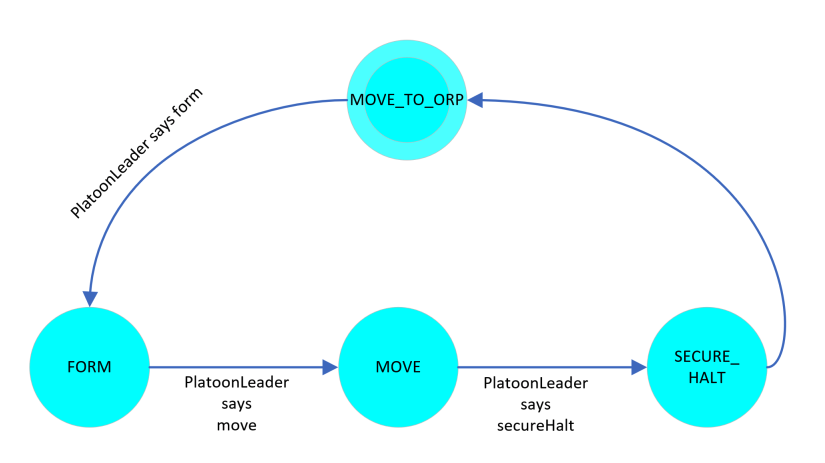
\includegraphics[width=0.8\textwidth]{../figures/ssmMoveToORPDiagram}
\caption{\label{ssmMoveToORPDiagram2} Horizontal slice: MoveToORP diagram.}
\end{figure}

Other than the number of principals, ssmMoveToORP follows the same structure as ssmPB described in the previous section.  

\subsection{Principals}
The principals are defined in the datatype stateRole.  



\subsection{States}
\HOLFreeVar{slState} = \HOLConst{MOVE_TO_ORP} \HOLTokenBar{} \HOLConst{PLT_FORM} \HOLTokenBar{} \HOLConst{PLT_MOVE} \HOLTokenBar{} \HOLConst{PLT_SECURE_HALT}
        \HOLTokenBar{} \HOLConst{COMPLETE}

\subsection{Outputs}
\HOLFreeVar{slOutput} = \HOLConst{MoveToORP} \HOLTokenBar{} \HOLConst{PLTForm} \HOLTokenBar{} \HOLConst{PLTMove} \HOLTokenBar{} \HOLConst{PLTSecureHalt}
         \HOLTokenBar{} \HOLConst{Complete} \HOLTokenBar{} \HOLConst{unAuthorized} \HOLTokenBar{} \HOLConst{unAuthenticated}

\subsection{Commands}

\HOLFreeVar{slCommand} = \HOLConst{pltForm} \HOLTokenBar{} \HOLConst{pltMove} \HOLTokenBar{} \HOLConst{pltSecureHalt} \HOLTokenBar{} \HOLConst{complete}
          \HOLTokenBar{} \HOLConst{incomplete}

\subsection{Next-State Function}
\subsection{Next-Output Function}
\subsection{Authentication}
\HOLThmTag{ssmPlanPB}{inputOK_def}\HOLssmPlanPBTheoremsinputOKXXdef


\HOLThmTag{PBIntegratedDef}{getOmniCommand_def}\HOLPBIntegratedDefTheoremsgetOmniCommandXXdef


\subsection{Authorization}
\subsection{Proved Theorems}



      %%%%%%%%%%%%%%%%%%% ssmPlanPB %%%%%%%%%%%%%%%%
\section{ssmPlanPB: Non-sequential Transitions}
The ssmPlanPB \glsentryshort{ssm} is one of the first \glsentryshortpl{ssm}\footnote{This is only partially true.  The first \glsentryshort{ssm} was ssmPB.  But, upon working with the \glsentryshort{ssm} in this section, the parametrizable ssm needed to updated to accommodate multiple input statements.  ssmPlanPB was the first \glsentryshort{ssm} used with this new parametrizable ssm.  All other \glsentryshortpl{ssm} were redone with the updated parametrizable ssm.}. It is the only \glsentryshort{ssm} that is not integrated with the Omni principal.  But, it is also the only \glsentryshort{ssm} that uses a non-sequential progression through states.  Figure \ref{ssmPlanPBDiagram2} is a diagram of this \glsentryshort{ssm}.

\begin{figure}[h!]
\centering
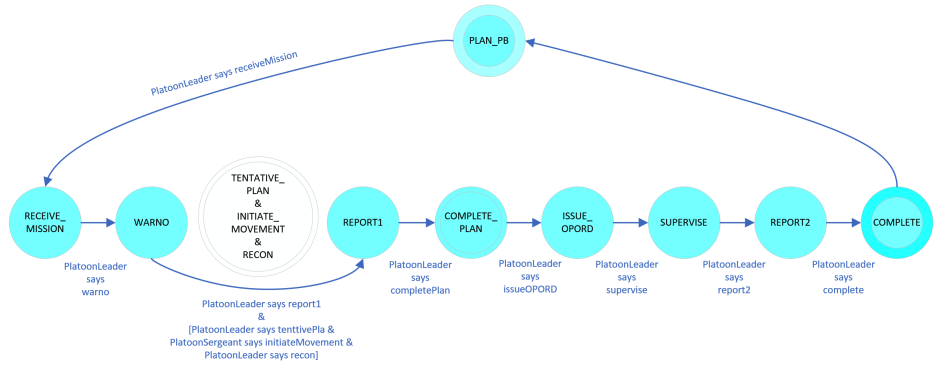
\includegraphics[width=\textwidth]{../figures/ssmPlanPBDiagram}
\caption{\label{ssmPlanPBDiagram2} Horizontal slice: PlanPB diagram.}
\end{figure}

The three non-sequential states are hidden in the white circle in the diagram.  They are TENTATIVE_PLAN, INITIATE_MOVEMENT, and RECON. These three states may be completed in any order, but all three must be completed before progressing to the next state REPORT1.  

To handle this, the three non-sequential states are combined into a "virtual state."  This state does not exist.  But, completion of these states must preceded transition from the WARNO state to the REPORT1 state.  Completion is indicated by the following three \glsentryshort{acl} statements
\[\text{\textit{PlatoonLeader says tentativePlan}}\]
\[\text{\textit{PlatoonSergeant says initiateMovement}}\]
\[\text{\textit{PlatoonLeader says recon}}\]


when combined with a request from the PlatoonLeader to transition to the REPORT1 state, the input for this transition is an input list with the four statements
\[\text{\textit{PlatoonLeader says tentativePlan}  }\]
\[\text{\textit{PlatoonSergeant says initiateMovement}  }\]
\[\text{\textit{PlatoonLeader says recon}}\]
\[\text{\textit{PlatoonLeader says report1}}\]

The security policy handles this with the following implication
\[\text{\textit{tentativePlan} andf  }\]
\[\text{\textit{initiateMovement} andf  }\]
\[\text{\textit{recon} impf}\]
\[\text{\textit{PlatoonLeader controls recon}}\]

The remaining details of this implementation follow.
\subsection{Principals}
The planning phase \glsentryshort{ssm} has two principals: PlatoonLeader and PlatoonSergeant.  These are defined in the \HOLFreeVar{stateRole} datatype.

\HOLFreeVar{stateRole} = \HOLConst{PlatoonLeader} \HOLTokenBar{} \HOLConst{PlatoonSergeant}

\subsection{States}
There are 12 states.  But, TENTATIVE_PLAN, INITIATE_MOVEMENT, and RECON are virtual states and not used in the next-state and next-output functions.

\begin{tabbing}
\parskip=8pt
\HOLFreeVar{slState} = \=\HOLConst{PLAN_PB} \\
				\>\HOLTokenBar{} \HOLConst{RECEIVE_MISSION} \\
				\>\HOLTokenBar{} \HOLConst{WARNO} \\
				\>\HOLTokenBar{} \HOLConst{TENTATIVE_PLAN}\\
        				\>\HOLTokenBar{} \HOLConst{INITIATE_MOVEMENT} \\
				\>\HOLTokenBar{} \HOLConst{RECON} \\
				\>\HOLTokenBar{} \HOLConst{REPORT1} \\
				\>\HOLTokenBar{} \HOLConst{COMPLETE_PLAN}\\
        				\>\HOLTokenBar{} \HOLConst{OPOID} \\
				\>\HOLTokenBar{} \HOLConst{SUPERVISE} \\
				\>\HOLTokenBar{} \HOLConst{REPORT2} \\
				\>\HOLTokenBar{} \HOLConst{COMPLETE}
\parskip=18pt
\end{tabbing}

\subsection{Commands}
The slCommand datatype for this \glsentryshort{ssm} is defined below.

\HOLFreeVar{slCommand} = \HOLConst{PL} \HOLTyOp{plCommand} \HOLTokenBar{} \HOLConst{PSG} \HOLTyOp{psgCommand}

The two datatypes for plCommand and psgCommand represent the PlatoonLeader and PlatoonSergeant commands, respectively. These are defined below.

\begin{tabbing}
\parskip=8pt
\HOLFreeVar{plCommand} = \=\HOLConst{receiveMission} \\
					     \>\HOLTokenBar{} \HOLConst{warno} \\
					     \>\HOLTokenBar{} \HOLConst{tentativePlan} \\
					     \>\HOLTokenBar{} \HOLConst{recon}\\
          				     \>\HOLTokenBar{} \HOLConst{report1} \\
				     	     \>\HOLTokenBar{} \HOLConst{completePlan} \\
					     \>\HOLTokenBar{} \HOLConst{opoid} \\
					     \>\HOLTokenBar{} \HOLConst{supervise} \\
					     \>\HOLTokenBar{} \HOLConst{report2}\\
          				     \>\HOLTokenBar{} \HOLConst{complete} \\
				     	     \>\HOLTokenBar{} \HOLConst{plIncomplete} \\
					     \>\HOLTokenBar{} \HOLConst{invalidPlCommand}
\parskip=18pt
\end{tabbing}

\begin{tabbing}
\parskip=8pt
\HOLFreeVar{psgCommand} = \=\HOLConst{initiateMovement} \\
						\>\HOLTokenBar{} \HOLConst{psgIncomplete}\\
           					\>\HOLTokenBar{} \HOLConst{invalidPsgCommand}
\parskip=18pt
\end{tabbing}

Providing each principal with her own set of commands simplifies the authentication and authorization functions.
\subsection{Output}
There are 14 outputs.  But, PlanPB, TentativePlan, InitiateMovement, and Recon are not used in the next-output function.  The unAuthorized output is returned for trapped commands.  The unAuthenticated output is returned for discarded commands.

\begin{tabbing}
\parskip=8pt
\HOLFreeVar{slOutput} =  \=\HOLConst{PlanPB} \\
					\>\HOLTokenBar{} \HOLConst{ReceiveMission} \\
					\>\HOLTokenBar{} \HOLConst{Warno} \\
					\>\HOLTokenBar{} \HOLConst{TentativePlan}\\
         				\>\HOLTokenBar{} \HOLConst{InitiateMovement} \\
					\>\HOLTokenBar{} \HOLConst{Recon} \\
					\>\HOLTokenBar{} \HOLConst{Report1} \\
					\>\HOLTokenBar{} \HOLConst{CompletePlan}\\
         				\>\HOLTokenBar{} \HOLConst{Opoid} \\
					\>\HOLTokenBar{} \HOLConst{Supervise} \\
					\>\HOLTokenBar{} \HOLConst{Report2} \\
					\>\HOLTokenBar{} \HOLConst{Complete}\\
         				\>\HOLTokenBar{} \HOLConst{unAuthenticated} \\
					\>\HOLTokenBar{} \HOLConst{unAuthorized}
\parskip=18pt
\end{tabbing}

\subsection{Next-State Function}
The next-state function takes the current state and a transition type and inputList pair.  It returns the next-state.  For the \textit{exec} transition type, an if-then-else decision statement checks the state and input.  If the input indicates a transition, then transition occurs, else no state change occurs.  The WARNO state is an exception.  It requires four inputs as described at the beginning of this section. To do this, four functions extract the appropriate command from the input list.  If all four commands are not present, then the else state returns WARNO (i.e., no state change occurs).

For the \textit{trap} and \textit{discard} transition types (the last two statements on the last line), the current state is returned for any command. 

\HOLThmTag{ssmPlanPB}{planPBNS_def}\HOLssmPlanPBTheoremsplanPBNSXXdef

Five functions are defined (see below) to extract the command from the input list.  These are getRecon, getTentativePlan, getReport, getInitMove, and getPlCom.  Each of these functions takes an input list as a parameter and returns a command with its option type.  For the sake of brevity, only getRecon is shown below.  The other functions are similar.

\paragraph*{HOL Definition for getRecon}...

\begin{lstlisting}
val getRecon_def = Define `
    (getRecon ([]:((slCommand command)option, stateRole, 'd,'e)Form list) =
    	      [NONE]) /\
    (getRecon ((Name PlatoonLeader) says (prop (SOME (SLc (PL recon))))
               :((slCommand command)option, stateRole, 'd,'e)Form::xs)
    	      	        = [SOME (SLc (PL recon)):(slCommand command)option]) /\
    (getRecon (_::xs) = getRecon xs)`
\end{lstlisting}

getRecon is defined recursively and uses pattern matching.  The first line beginning with getRecon pattern matches against an empty list of type \textit{((slCommand command)option, stateRole, 'd,'e)Form list)} as input.  It returns the option type NONE.  The next getRecon pattern matches the head of the list with \textit{((Name PlatoonLeader) says (prop (SOME (SLc (PL recon))))} of type  \textit{((slCommand command)option, stateRole, 'd,'e)Form list)}.  This returns \textit{[SOME (SLc (PL recon)):(slCommand command)option]}.  The final getRecon pattern matches the wild card "_" to any other input.  It recursively calls getRecon on the remainder of the list, while throwing out the head.

\paragraph*{HOL Generated Output for getRecon}...
The \glsentryshort{hol} generated code converts the wild card into all allowable cases for head of the list.  It is shown below.

\HOLThmTag{PlanPBDef}{getRecon_def}\HOLPlanPBDefTheoremsgetReconXXdef

\subsection{Next-Output Function}
The next-output differs from the next-state function in that it returns an output rather than a state.  It follows the same logic.  The \textit{trap} and \textit{discard} transition types return the outputs unAuthorized and unAuthenticated, respectively.
\HOLThmTag{ssmPlanPB}{planPBOut_def}\HOLssmPlanPBTheoremsplanPBOutXXdef


\subsection{Authentication}
The authenticationTest function takes an elementTest function and an input list as parameters.  authenticationTest is defined in the parametrizable ssm.  elementTest function is defined as a parameter in each \glsentryshort{ssm}.  In the \glsentryshortpl{ssm}, elementTest is named inputOK.  

\paragraph*{HOL Definition for inputOK}

The \glsentryshort{hol} definition for inputOK uses the wild card "_".  Thus, the \glsentryshort{hol} definition differs from the \glsentryshort{hol} generated output.  The \glsentryshort{hol} definition is shown below. 

\begin{lstlisting}
val inputOK_def = Define
`(inputOK
	(((Name PlatoonLeader) says (prop  (cmd:((slCommand command)option))))
	       :((slCommand command)option, stateRole, 'd,'e)Form) = T)  /\
(inputOK
	(((Name PlatoonSergeant) says (prop  (cmd:((slCommand command)option))))
	       :((slCommand command)option, stateRole, 'd,'e)Form) = T)  /\
(inputOK _ = F)`
\end{lstlisting}

inputOK uses pattern matching, but not recursion.  The first inputOK pattern matches the input against \textit{(((Name PlatoonLeader) says (prop  (cmd:((slCommand command)option))))} which is of type \textit{((slCommand command)option, stateRole, 'd,'e)Form)}.  This is defined as T (True).  This authenticates the PlatoonLeader on any slCommand.  The next inputOK pattern matches the input against \textit{((Name PlatoonSergeant) says (prop  (cmd:((slCommand command)option))))} which is of the same type as the first pattern.  This is defined as T (True).  This authenticates the PlatoonSergeant on any slCommand.  The last inputOK pattern uses the wild card to match ANY OTHER input.  ANY OTHER input is defined as F (false).
	 
	 
\paragraph*{HOL Generated Output for inputOK}

The \glsentryshort{hol} generated output matches the wild card to all other possible values for the input.

\HOLThmTag{ssmPlanPB}{inputOK_def}\HOLssmPlanPBTheoremsinputOKXXdef

The theorem inputOK_cmd_reject_lemma proves that any command that is not requested by a principal is false.

\begin{lstlisting}
val inputOK_cmd_reject_lemma =
TAC_PROOF(
  ([],
   ``!cmd. ~(inputOK
   	   ((prop (SOME cmd)):((slCommand command)option, stateRole, 'd,'e)Form))``),
  PROVE_TAC[inputOK_def])
\end{lstlisting}


\subsection{Authorization}
Authorization is defined in two ways.  Authorization is state-dependent because of the added requirement for the transition from the WARNO state to the REPORT1 state.  This is equivalent to the stateInterp function in ssm.  In ssmPlanPB, this function is called secContext.

\begin{lstlisting}
val secContext_def = Define `
secContext (s:slState) (x:((slCommand command)option, stateRole, 'd,'e)Form list) =
    if (s = WARNO) then
        (if (getRecon         x = [SOME (SLc (PL recon))
                                   :(slCommand command)option] ) /\
	    (getTenativePlan  x = [SOME (SLc (PL tentativePlan))
	    		      	   :(slCommand command)option]) /\
            (getReport        x = [SOME (SLc (PL report1))
	    		      	   :(slCommand command)option]) /\
	    (getInitMove      x = [SOME (SLc (PSG initiateMovement))
	    		      	   :(slCommand command)option])
         then [
	       PL_WARNO_Auth
	        :((slCommand command)option, stateRole, 'd,'e)Form;
		(Name PlatoonLeader) controls prop (SOME (SLc (PL recon)));
		(Name PlatoonLeader) controls prop (SOME (SLc (PL tentativePlan)));
	       (Name PlatoonSergeant) controls prop (SOME (SLc (PSG initiateMovement)))]
	 else [(prop NONE):((slCommand command)option, stateRole, 'd,'e)Form])
    else if ((getPlCom x) = invalidPlCommand)
    	 then [(prop NONE):((slCommand command)option, stateRole, 'd,'e)Form]
	 else [PL_notWARNO_Auth (getPlCom x)]`
\end{lstlisting}

secContext uses pattern matching, but not recursion. It is similar to the definition for the next state function.  If the \textit{s = WARNO}, then secContext looks for all four statements using the get* functions.   If these are all present, then secContext returns \textit{PL_WARNO_Auth}. \textit{PL_WARNO_Auth} contains the implication that authorizes the Platoon Leader on the transition to REPORT1.  If all four statements are not present, then \textit{ [(prop NONE)]} is returned.


\begin{lstlisting}
val PL_WARNO_Auth_def = Define `
    PL_WARNO_Auth =
    ^(impfTermList
    [``(prop (SOME (SLc (PL recon))))
         :((slCommand command)option, stateRole, 'd,'e)Form``,
     ``(prop (SOME (SLc (PL tentativePlan))))
         :((slCommand command)option, stateRole, 'd,'e)Form``,
     ``(prop (SOME (SLc (PSG initiateMovement))))
         :((slCommand command)option, stateRole, 'd,'e)Form``,
     ``(Name PlatoonLeader) controls prop (SOME (SLc (PL report1)))
         :((slCommand command)option, stateRole, 'd,'e)Form``]
     ``:((slCommand command)option, stateRole, 'd,'e)Form``)`
\end{lstlisting}

The remainder of secContext applies to all other states.  If the getPlCom function returns \textit{invalidPlComand}, then secContext returns  \textit{ [(prop NONE)]} is returned.  Otherwise, it returns \textit{PL_notWARNO_Auth}.  \textit{PL_notWARNO_Auth} authorizes the PlatoonLeader on any plCommand except \textit{report1}. If the command is \textit{report1} is found, then it returns \textit{ [(prop NONE)]}.

\begin{lstlisting}
val PL_notWARNO_Auth_def = Define `
    PL_notWARNO_Auth (cmd:plCommand) =
    if (cmd = report1) (* report1 exits WARNO state *)
    then
      (prop NONE):((slCommand command)option, stateRole, 'd,'e)Form
    else
      ((Name PlatoonLeader) says (prop (SOME (SLc (PL cmd)))
       :((slCommand command)option, stateRole, 'd,'e)Form) impf
      (((Name PlatoonLeader) controls prop (SOME (SLc (PL cmd))))
      :((slCommand command)option, stateRole, 'd,'e)Form)) `
\end{lstlisting}

\subsection{Proved Theorems}
The following theorems prove various properties about the \glsentryshort{ssm}.  Descriptions are similar to those of previously described \glsentryshortpl{ssm}.  


\paragraph*{PlatoonLeader_notWARNO_notreport1_exec_plCommand_justified_thm}
This theorem proves that if the state is NOT WARNO and the PlatoonLeader issues any plCommand other than \textit{report1}, then that command should be executed.  Two lemmas are required first.

\HOLThmTag{ssmPlanPB}{PlatoonLeader_notWARNO_notreport1_exec_plCommand_lemma}\HOLssmPlanPBTheoremsPlatoonLeaderXXnotWARNOXXnotreportOneXXexecXXplCommandXXlemma

\HOLThmTag{ssmPlanPB}{PlatoonLeader_notWARNO_notreport1_exec_plCommand_justified_lemma}\HOLssmPlanPBTheoremsPlatoonLeaderXXnotWARNOXXnotreportOneXXexecXXplCommandXXjustifiedXXlemma

\HOLThmTag{ssmPlanPB}{PlatoonLeader_notWARNO_notreport1_exec_plCommand_justified_thm}\HOLssmPlanPBTheoremsPlatoonLeaderXXnotWARNOXXnotreportOneXXexecXXplCommandXXjustifiedXXthm

\paragraph*{PlatoonLeader_psgCommand_notDiscard_thm}
This next theorem proves that if the PlatoonLeader issues a psgCommand then that command is not discarded.  The reason for this is that the psgCommand is an slCommand.  In inputOK, the PlatoonLeader is authenticated on all psgCommand.  Therefore, this command should be trapped an not discarded.

\HOLThmTag{ssmPlanPB}{PlatoonLeader_psgCommand_notDiscard_thm}\HOLssmPlanPBTheoremsPlatoonLeaderXXpsgCommandXXnotDiscardXXthm


\paragraph*{PlatoonSergeant_trap_plCommand_justified_thm}
This next theorem proves that if the PlatoonLeader issues a psgCommand then that command is trapped.  It requires two lemmas.

\HOLThmTag{ssmPlanPB}{PlatoonLeader_trap_psgCommand_lemma}\HOLssmPlanPBTheoremsPlatoonLeaderXXtrapXXpsgCommandXXlemma

\HOLThmTag{ssmPlanPB}{PlatoonLeader_trap_psgCommand_justified_lemma}\HOLssmPlanPBTheoremsPlatoonLeaderXXtrapXXpsgCommandXXjustifiedXXlemma

\HOLThmTag{ssmPlanPB}{PlatoonSergeant_trap_plCommand_justified_thm}\HOLssmPlanPBTheoremsPlatoonSergeantXXtrapXXplCommandXXjustifiedXXthm

\paragraph*{PlatoonLeader_WARNO_exec_report1_justified_thm}
This theorem proves that if the state IS WARNO and the PlatoonLeader issues the plCommand \textit{report1}, then that command should be executed.  Two lemmas are required first.  

Notice that the 

\HOLThmTag{ssmPlanPB}{PlatoonLeader_WARNO_exec_report1_lemma}\HOLssmPlanPBTheoremsPlatoonLeaderXXWARNOXXexecXXreportOneXXlemma

\HOLThmTag{ssmPlanPB}{PlatoonLeader_WARNO_exec_report1_justified_lemma}\HOLssmPlanPBTheoremsPlatoonLeaderXXWARNOXXexecXXreportOneXXjustifiedXXlemma

\HOLThmTag{ssmPlanPB}{PlatoonLeader_WARNO_exec_report1_justified_thm}\HOLssmPlanPBTheoremsPlatoonLeaderXXWARNOXXexecXXreportOneXXjustifiedXXthm


\paragraph*{PlatoonSergeant_trap_plCommand_justified_thm}
This theorem proves that the PlatoonSergeant is trapped on all plCommands.  It requires two lemmas.

\HOLThmTag{ssmPlanPB}{PlatoonSergeant_trap_plCommand_lemma}\HOLssmPlanPBTheoremsPlatoonSergeantXXtrapXXplCommandXXlemma

\HOLThmTag{ssmPlanPB}{PlatoonSergeant_trap_plCommand_justified_lemma}\HOLssmPlanPBTheoremsPlatoonSergeantXXtrapXXplCommandXXjustifiedXXlemma

\HOLThmTag{ssmPlanPB}{PlatoonSergeant_trap_plCommand_justified_thm}\HOLssmPlanPBTheoremsPlatoonSergeantXXtrapXXplCommandXXjustifiedXXthm


\end{document}